\documentclass[10pt,a4paper,titlepage]{book}
\usepackage[ukrainian]{babel}
\documentclass[10pt,a4paper,titlepage]{book}
%\documentclass[12pt,b5paper,titlepage]{book}
%\documentclass[10pt,a4paper,titlepage,twocolumn]{book}
\usepackage[utf8]{inputenc}
\usepackage{cmap}
\usepackage[ukrainian]{babel}
\usepackage[OT1]{fontenc}
\usepackage{amsmath}
\usepackage{amsfonts}
\usepackage{amssymb}
\usepackage{amsthm}
\usepackage{graphicx}
\usepackage{indentfirst}
\usepackage{bbm}
\usepackage{mathtools}
%\usepackage{index}
\usepackage{makeidx}
%\usepackage{showidx} % Show indeces on pages
\usepackage[
    unicode=true,
    breaklinks,
    colorlinks=true,
    linkcolor=blue,
    ]{hyperref}
\usepackage{enumitem}
\usepackage{verbatim}
\usepackage{framed}
\usepackage{pstricks}
\usepackage{cancel} % formulas cancel
\usepackage{multicol}
\author{Завадська Л.О., Савчук М.М.}

\pdfcompresslevel=9

\everymath{\displaystyle}

\theoremstyle{plain}
%\newtheorem{affirmation}{Утверждение}[section]
\newtheorem{theorem}{Теорема}[chapter]
%\newtheorem{lemma}{Лемма}[section]
\newtheorem{remark}{Зауваження}

\theoremstyle{definition}
\newtheorem{definition}{Визначення}[chapter]
\newtheorem{example}{Приклад}[chapter]

\theoremstyle{remark}

%\newcommand{\stcomp}[1]{{#1'}}
\newcommand{\stcomp}[1]{\overline{#1}}
\newcommand{\Probability}[1]{\mathbb{P}\left\{ #1 \right\}}
\newcommand{\probability}[1]{\mathbb{P}\left( #1 \right)}
\newcommand{\probabilityn}[1]{\mathbb{P}_n\left( #1 \right)}
\newcommand{\indicator}[1]{\mathbbm{1}\left( #1 \right)}
\newcommand{\Indicator}[1]{\mathbbm{1}\left\{ #1 \right\}}
\newcommand{\indicatorof}[1]{\mathbbm{1}_{#1}}
\newcommand{\meanof}[2]{M_{#1} #2}
\newcommand{\dispersionof}[2]{D_{#1} #2}
\newcommand{\dispersion}[1]{\dispersionof{}{#1}}
\newcommand{\mean}[1]{\meanof{}{#1}}
\newcommand{\covergence}[1]{\xrightarrow[n\to\infty]{#1}}
\newcommand{\Covergence}[1]{\xRightarrow[n\to\infty]{#1}}
\newcommand{\covergencen}[2]{\xrightarrow[#1\to\infty]{#2}}
\def \probabilityCovergenceText {\mathbb{P}}
\newcommand{\pcovergence}{\covergence{\probabilityCovergenceText}}
\newcommand{\pCovergence}{\Covergence{\probabilityCovergenceText}}
\def \almostSureCovergenceText {a.s.}
\newcommand{\acovergence}{\covergence{\almostSureCovergenceText}}
\newcommand{\aCovergence}{\Covergence{\almostSureCovergenceText}}
\def \distributionCovergenceText {d}
\newcommand{\dcovergence}{\covergence{\distributionCovergenceText}}
\newcommand{\dCovergence}{\Covergence{}}
\newcommand{\cdfof}[2]{F_{#1}\left(#2\right)}
\newcommand{\cdf}[1]{\cdfof{}{#1}}
\newcommand{\cdfn}[1]{F_n\left(#1\right)}
\newcommand{\CDFOF}[2]{F_{#1}\left\{#2\right\}}
\newcommand{\CDF}[1]{\CDFOF{}{#1}}
\newcommand{\pdf}[1]{p\left(#1\right)}

\newcommand{\integralc}[4]{\int\limits_{#1}^{#2} #4 #3}
\newcommand{\integral}[4]{\integralc{#1}{#2}{d #3}{#4}}
\newcommand{\integralp}[4]{\integralc{#1}{#2}{\partial #3}{#4}}

\newcommand{\argmaxof}[2]{\underset{#2}{\operatorname{arg\,max}}#1}
\newcommand{\argmax}[1]{\argmaxof{#1}{}}

\renewcommand{\thefootnote}{\fnsymbol{footnote}} 

%\renewcommand{\thesection}{Лекція \arabic{section}}
%\usepackage{titlesec}
%\titleformat{\section}{\normalfont\bfseries}{\thesection}{0.5em}{}
%\titleformat{\subsection}{\itshape}{}{0.5em}{}
%\titleformat{\subsection}{\normalfont\textit}{\thesubsection}{0.5em}{}

\pagestyle{empty} % Empty page header

\author{Завадська Л.О., Савчук М.М.}

\theoremstyle{plain}
%\newtheorem{affirmation}{Утверждение}[section]
\newtheorem{theorem}{Теорема}[chapter]
%\newtheorem{lemma}{Лемма}[section]
\newtheorem{remark}[theorem]{Зауваження}

\theoremstyle{definition}
\newtheorem{definition}[theorem]{Визначення}
\newtheorem{example}[theorem]{Приклад}

\title{Математичні методи захисту інформації: курс лекцій. Частина 1}

\makeindex
\begin{document}

\maketitle

\chapter{Задачі, напрямки та методи захисту інформації.
    Поняття про криптографічний захист інформації}\label{lecture:1}
\section{Області застосування, мета, методи захисту інформації}
Протягом свого існування людство пережило декілька інформаційних революцій:
створення і розвиток мов, винахід писемності, винахід та широке застосування
друкарства, створення комп’ютера та новітніх електронних технологій, що
радикально змінили суспільство в усіх галузях, на всіх рівнях  суспільного
розвитку. Кількість інформації, що була доступна та використовувалась, постійно
зростала, а за періоди інформаційних революцій --- на декілька порядків.
Володіння інформацією і в минулому і нині давало можливість досягти швидкого
розвитку і успіху у різних галузях як у глобальному масштабі, так і в
конкретних справах. Сьогодні світ переживає період, коли накопичено колосальний
об’єм знань, що  дозволяє перейти до здійснення справді революційних
технологічних рішень. Основою розвитку  нині може бути, перш за все, процес
пізнання, і він посильний тільки високоосвіченому суспільству, в якому праця
приймає все більш інтелектуальні форми. Технологіям майбутнього потрібні широко
освічені люди, які здатні орієнтуватися в нових умовах дійсності, що стрімко
змінюється.

Однією з галузей, що  найбільш динамічно  змінюються  протягом останніх
десятиліть, є технології електронної обробки інформації, телекомунікацій,
комп’ютерних мереж, технології захисту інформації.

В Україні широкий попит на методи і засоби захисту інформації почав виявлятися у
другій половині 80-х років ХХ ст. З часом виникла нагальна потреба використання
криптографічних та технічних методів захисту також у приватному секторі.
Сьогодні велика кількість конфіденційної інформації передається в електронному
вигляді, на електронних носіях, між ЕОМ звичайними лініями зв’язку. Інформація
може продаватися та купуватися, мати ціну, що незрівнянно перевищує ціну
матеріального носія. Часто володіння інформацією дає переваги, ціну яких
неможливо підрахувати, наприклад, у військовій справі. Термін збереження
секретності інформації може коливатися від декількох годин до багатьох
десятиліть. Тому вкрай потрібні спеціалісти, які володіють  криптографічними,
технічними, комплексними методами захисту, знають відповідні стандарти, здатні
використовувати (або розробляти) програмне й апаратне забезпечення для
гарантування таємності та цілісності конфіденційної інформації. Криптографічні
методи захисту вважаються одними з найбільш надійних та ефективних. 

\begin{itemize}
    \item{Області застосування захисту інформації
        (відповідно --- види таємниці):}
        \begin{multicols}{2}
            \begin{enumerate}
                \item Військова;
                \item Дипломатична;
                \item Фінансова;
                \item Банківська;
                \item Комерційна;
                \item Промислова;
                \item Наукова;
                \item Юридична;
                \item Медична;
                \item Особиста таємниця.
            \end{enumerate}
        \end{multicols}
    \item{Мета і головні задачі захисту інформації:}
        \begin{enumerate}
            \item Конфіденційність (секретність) інформації;
            \item Цілісність інформації;
            \item Автентичність інформації;
            \item Доступність інформації.
        \end{enumerate}
    \item{Напрямки, аспекти, методи і засоби захисту інформації:}
        \begin{enumerate}
        \item Юридичні, правові;
        \item Методично-нормативні;
        \item Організаційні;
        \item Безпосередні (фізичні);
        \item Технічні --- захист від витоку  по технічним каналам:
            \begin{enumerate}
                \item електромагнітному
                \item оптичному
                \item акустичному
                \item віброакустичному;
        \end{enumerate}
        \item Стеганографічні;
        \item Криптографічні. Методи математичного захисту інформації; 
        \item Методи квантової криптографії; 
        \item Морально-етичні норми.  
    \end{enumerate}
\end{itemize}
\section{Перші поняття криптографічного  захисту інформації}

\begin{definition}[Криптографічний захист інформації]
    Криптографічний захист інформації --- це різновид
    захисту інформації, який реалізується за допомогою криптографічних перетворень,
    спеціальних ключових даних з метою приховування та відновлення змісту
    інформації, підтвердження достовірності, авторства, запобігання
    несанкціонованому використанню тощо.
\end{definition}

\begin{definition}[Криптографічне перетворення]
    Криптографічне перетворення --- це перетворення
    інформації відповідно до певних правил (логічних, математичних) з метою
    забезпечення функціонування криптографічних протоколів.
\end{definition}

\begin{definition}[Криптографічний ключ]
    Криптографічний ключ --- це параметр, який
    використовується в криптографічному алгоритмі для вибору конкретного
    криптографічного перетворення; ключі можуть бути таємними або відкритими.
\end{definition}

\begin{definition}[Криптографічний протокол]
    Криптографічний протокол --- це послідовність
    узгоджених дій згідно з деякими правилами, у відповідності з якими відбувається
    обмін інформацією між сторонами або учасниками протоколу та її перетворення з
    використанням криптографічних методів і засобів.  Простий приклад
    криптографічного протоколу – це зашифрування та розшифрування повідомлення.
\end{definition}

\begin{definition}[Криптографія]
    Криптографія --- науково-технічна дисципліна, яка
    вивчає принципи, методи і засоби криптографічного захисту інформації і
    інформаційних технологій, предметом якої є розробка криптографічних систем.
\end{definition}

\begin{definition}[Криптоаналіз]
    Криптоаналіз --- це науково-технічна дисципліна, яка
    вивчає методи, способи і засоби аналізу криптографічного захисту інформації:
    криптографічних систем, криптографічних алгоритмів, протоколів з метою знайти
    способи їх розкриття без знання секретних ключів і, можливо, будови
    криптосистем, знайти способи несанкціонованого доступу, підробки даних тощо.
    Криптоаналіз оцінює складність таких способів  розкриття (злому) і стійкість
    криптографічного захисту інформації. Фахівця, який займається криптоаналізом
    будемо називати криптоаналітиком.
\end{definition}

\begin{definition}[Криптологія]
    Криптологія за найбільш поширеною сучасною
    термінологією, об'єднує в собі дисципліни криптографію і
    криптоаналіз.
\end{definition}

\begin{remark}
    Не всі  країни дотримуються останньої термінології щодо
    дисциплін. Так, наприклад, в Росії назва „криптографія” об’єднує в собі власне
    криптографію (криптосинтез) у вище наведеному розумінні і криптоаналіз, а
    криптологія розглядається як галузь криптографії, що вивчає математичні моделі
    криптографічних систем, і також поділяється на криптосинтез та криптоаналіз.
\end{remark}
\section{Етапи розвитку технологічних засобів  криптографії}
\begin{enumerate}
    \item ``Ручна'' криптографія (із давнини до середини-кінця XIX століття)

        Основні види шифрів --- заміни і перестановки.

        \begin{figure}[hb]
            \centering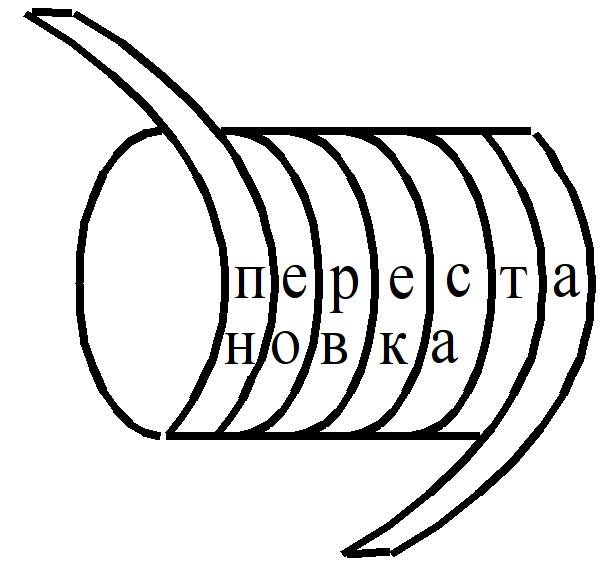
\includegraphics[width=1.0in]{crypt-img/crypt-img1.png}
            \caption{Шифр Скитала}\label{scitalCipher}
        \end{figure}

        Перший шифр перестановки,
        застосування якого зафіксоване у військовій справі,
        (Спарта, V ст. до н.е.) – шифр Скитала (рис. \ref{scitalCipher}).
        Таємний ключ – діаметр барабана.

        \begin{figure}[hb]
            \centering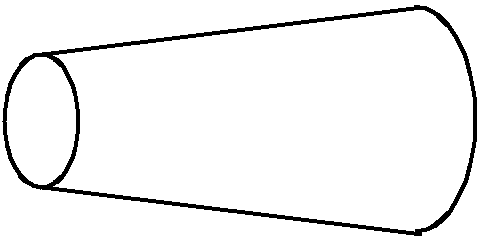
\includegraphics[width=1.0in]{crypt-img/crypt-img2.png}
            \caption{Засіб криптоаналізу шифру Скитала}\label{scitalAnalysis}
        \end{figure}

        Для  шифрування на стрічці, що намотувалась на барабан (скитал),
        писалось вздовж барабана повідомлення.
        Після знімання з барабану на стрічці була зовні
        випадкова послідовність літер – шифроване повідомлення.
        Криптоаналіз шифру Скитала запропонував Арістотель
        за допомогою барабана змінного діаметру (рис. \ref{scitalAnalysis}):
        якщо на намотаній на нього стрічці з шифрованим повідомленням у
        деякому місці вгадувались якісь частини слів,
        то цьому місцю відповідав діаметр справжнього барабану. 

        Прикладом шифру заміни є шифр Цезаря --- заміна кожної букви
        повідомлення на букву  циклічно віддалену
        в алфавіті на фіксоване число позицій.
    \item Застосування телеграфу для шифрування і кодування (з середини XIX ст.)
    \item Використання механічних машин (кінець XIX ст. – 20і роки XX ст.)
    \item Електромеханічні машини (з 20-х років XX ст. – середина XX ст.)

        Приклад --- ENIGMA --- основна шифрувальна машина Вермахту
        у Другій світовій війні.
    \item Електронні машини (з кінця 40-х років XX ст.)
    \item Напівпровідникові криптосистеми
    \item Криптосистеми, засновані на мікросхемах
    \item Використання комп'ютерної техніки для криптографічного захисту
    \item Квантова криптографія
\end{enumerate}

\section{Про розвиток теоретичної криптографії}

До епохи Відродження криптографією займалися, можна сказати, не професіонали.
Найчастіше шифри уявляли  собою деякі головоломки. Але слід зазначити, що іноді
винаходилися шифри, які не були розкриті на протязі  100 і навіть більше років!
Хоча за сучасними  поняттями,  враховуючи залучення до криптоаналізу ЕОМ,
загалом це були  слабкі, нестійкі шифри.

Велике просування в криптографії відбулося після залучення до вирішення її
проблем  відомих математиків періоду відродження, серед яких  були Ф. Вієт, Д.
Кардано та ін. Пізніше почали створюватись спеціалізовані державні служби
шифрування і дешифрування (розкриття). Такі служби створили, наприклад,
Кромвель у Англії, кардинал Рішельє у Франції, Петро I  в Росії. 

У 1883 році була опублікована  книга Керкгоффа «Військова криптографія», в якій 
були вперше сформульовані деякі вимоги до криптосистем, правила щодо утворення,
експлуатації, стійкості  криптографічних пристроїв. Частина цих правил і зараз
вважаються обов'язковими. 

Наукою у повному розумінні цього слова теоретичну  криптографію стали визнавати
з 1949 року після публікації у відкритому друці  статті К. Шеннона ``Теорія
зв'язку в секретних системах''. А з 1976 року завдяки ідеям
статті  Діффі і Хеллмана ``Нові напрямки в криптографії'' почався новий  етап у
розвитку  криптографії – застосування криптосистем з відкритим ключем, яке дало
можливість успішно вирішити низку назрілих  проблем криптографічного захисту
інформації.

\section{Класифікація сучасних  криптосистем}

\begin{enumerate}
    \item \textit{Симетричні (одноключові, з секретним ключем).}
        Підрозділяються на блокові й потокові.
        У відправника та одержувача повідомлення один і той самий
        секретний ключ, вони знаходяться у рівних (симетричних) умовах,
        можуть як зашифрувати повідомлення так і  розшифрувати
        за допомогою таємного ключа.
    \item \textit{Асиметричні (двохключові, з відкритим ключем, із
        загальнодоступними ключами).}
        Відомі з 1976 року, активно використовуються на практиці з 1978 року.
        У найпростішому випадку мають два ключі: один (відкритий)
        --- у відправника для шифрування, інший --- у одержувача (секретний) для
        розшифрування.
    \item \textit{Квантові} (знаходяться у стадії експерименту та розвитку)
\end{enumerate}

\section{Контрольні питання}
\begin{enumerate}
    \item Які  мета та задачі захисту інформації?
    \item Назвіть напрямки та методи захисту інформації.
    \item Що таке криптографічний ключ?
    \item З яких частин складається криптологія?
    \item Чи були відомі способи захисту інформації шифруванням до нашої ери?
    \item Коли використовувались роторні шифрувальні машини?
    \item Яка дата вважається початком розвитку криптографії
        з відкритим  ключем?
    \item Чим відрізняються симетричні криптосистеми від асиметричних?
\end{enumerate}

\chapter{Моделі джерел відкритого тексту. Ентропія на символ джерела}
\label{lecture:2}

При шифруванні текст перетворюється таким чином, щоб зробити його зміст
незрозумілим для того, хто не знає секретного ключа. Для побудови математичної
теорії криптографічних систем шифрування потрібно насамперед дати математичний
опис (або математичну модель) тексту та перетворень, які відбуваються з ним під
час шифрування.

\begin{definition}[Алфавіт]
    Надалі вважатимемо, що алфавіт є скінченним.
    Позначимо алфавіт як $Z_m = \left\{z_1, \dots , z_m \right\}$, де
    $z_1, \dots , z_{m}$ --- букви (символи) алфавіту.
    Елементами алфавіту можуть бути власне букви; букви та цифри;
    букви, цифри та знаки пунктуації, взагалі скінченний набір
    будь-яких символів, наприклад, танцюючі чоловічки.
    Як правило, ми будемо розглядати український,
    російський чи латинський алфавіт (малі букви) зі знаком пропуску,
    що вважається буквою, або без нього, або ж двійковий алфавіт,
    що складається з двох символів: $0$ та $1$. 
\end{definition}
\begin{definition}[Текст]
    Під текстом будемо розуміти послідовність букв деякого алфавіту.
\end{definition}

\begin{definition}[Відкритий текст] Відкритий текст (ВТ) --- це текст,
    що підлягає шифруванню.
\end{definition}
\begin{definition}[Шифрований текст]Шифрований текст (ШТ) --- це текст,
    що утворюється в результаті шифрування.
\end{definition}

Відкритий та шифрований тексти можуть бути записані як у одному й тому ж,
так і у різних алфавітах (більш докладно поняття ВТ та ШТ
розглядаються у лекції 3).

\begin{definition}[n-грама]
n-грамою називається послідовність  $n$ символів тексту, що
стоять підряд. При  ${n}$=2 це біграма, при  ${n}$=3 --- триграма.
\end{definition}

Будь-який текст має певну статистичну структуру. Для опису цієї структури
використовуються різноманітні ймовірнісні моделі мови. 

\begin{definition}[Джерело відкритого тексту]
    Джерело відкритого тексту генерує послідовність символів алфавіту 
    $x_1, x_2, \dots, x_n, \dots$ випадковим чином.
    Джерело визначається алфавітом та ймовірностями появи $n$-грам: 
    $\probability{x_{i+1}=z_1, x_{i+2}=z_2, \dots, x_{i+n}=z_n}$
    для будь-яких цілих  $n \ge 1$, $i \geq 0$
    (тут $x_1, x_2, \dots, x_n$ --- випадкові величини,
    а $z_1, \dots, z_n$ --- букви алфавіту), які мають задовольняти умовам: 

    \begin{enumerate}
        \item Вихід джерела ВТ є випадковим процесом
            з дискретним часом та множиною станів  $Z_m$
        $$\sum_{z_1, z_2, \dots, z_n \in Z_m}
            \probability{x_{i+1}=z_1, \dots, x_{i+n}=z_n}=1$$
        \item Умова узгодженості
            скінченновимірних розподілів виходу джерела ВТ:
            Для будь-якого цілого  ${s\ge 1}$
        \begin{align*}
            \sum_{z_1, z_2, \dots, z_n \in Z_m}
                \probability{x_{i+1}=z_1, \dots, x_{i+n}=z_n, \dots, x_{i+n+s}
                    =z_{n+s}} = \\
                = \probability{x_{i+1}=z_1, \dots, x_{i+n}=z_n}
        \end{align*}
    \end{enumerate}
\end{definition}

\begin{definition}[Стаціонарне джерело відкритого тексту]
    Джерело називають стаціонарним, якщо для будь-яких цілих  $n\ge 1,
    1\le i_1<\dots<i_n,j\ge 0$
    і будь-якого набору букв алфавіту  $z_1, \dots,z_n$ виконується  рівність:
    $$\probability{x_{i_1+j}=z_1, x_{i_2+j}=z_2, \dots, x_{i_n+j}=z_n}
        = \probability{x_{i_1}=z_1, x_{i_2}=z_2, \dots, x_{i_n}=z_n}$$
\end{definition}

У подальшому будемо розглядати лише стаціонарні джерела, тобто такі, у яких
немає залежності від зсуву $j$.
Для стаціонарних джерел достатньо задати ймовірності
$\probability{x_1=z_1,\dots,x_n=z_n}$ для ${n\ge 1}$.

В залежності від властивостей сумісних розподілів 
$\probability{x_1=z_1, \dots, x_n=z_n}$, $n\ge 1$
можна побудувати різні моделі джерела ВТ.

Найбільш уживаними є описані нижче чотири моделі, з яких кожна наступна все
більш адекватно відображає структуру мови. Перша з них є простою й менш за всі
враховує реальні статистичні властивості мови. Назвемо її моделлю М0.
\begin{definition}[Модель M0]
    У цій моделі джерело у кожен момент часу генерує символи
    із  $Z_m$ незалежно та рівноімовірно:
    $$\probability{x_i=z}=\frac{1}{m}, z \in Z_m, i = 1, 2, \dots$$

    Всі  $n$-грами в моделі М0 є рівноймовірними
    для  будь-яких цілих  ${n\ge 1}$ та
    $z_1,\dots,z_n \in Z_m$
    $$\probability{x_1=z_1,\dots,x_n}=z_{{n}}=\frac{1}{m^n}$$

    Модель М0 має допоміжний характер,
    бо вона не враховує навіть найпростіших властивостей мови.
\end{definition}

Наступна модель ВТ враховує частоти, з якими окремі букви зустрічаються у мові.

\begin{definition}[Модель M1]
    Символи тексту  $x_1, x_2, \dots, x_n, \dots$ є
    незалежними, але вони генеруються із різними ймовірностями
    $$\probability{x_i=z}=\pdf{z}, z \in Z_m, i=1, 2, \dots$$

    Розподіл ймовірностей  $\pdf{z}$ відповідає частотам появи букв  $z \in Z_m$
    у мові. У цій моделі ймовірність появи n-грами має вигляд:

    $$\probability{x_1=z_1, x_2=z_2, \dots, x_n=z_n}
        = \prod_{i=1}^n \pdf{z_i}$$

    Зазначимо, що ймовірності букв у природних мовах значно відрізняються.
    Наприклад,
    найбільшу частоту в українській та російській мові має буква “о”,
    в англійській --- буква ``e''.
    В російській мові ``о'' зустрічається майже в 50 раз частіше букви ``ф'',
    що має найменшу частоту.\footnote{За умови,
    що твердий знак ототожнюється з м’яким.}
\end{definition}

Наступна модель враховує залежність в мові між двома буквами, що стоять поряд.

\begin{definition}[Модель M2]
    Джерело генерує біграми $x_1 x_2, x_3 x_4, x_5 x_6, \dots$ і
    т.д. незалежно одну від одної.
    Тобто на множині всіх біграм заданий розподіл імовірностей
    $\pdf{z_i, z_j}, i, j = 1 , \dots ,m$, і кожна
    нова біграма джерела генерується незалежно від інших.
\end{definition}

Більш складні залежності мови враховуються за допомогою марковської моделі.

\begin{definition}[Однорідний ланцюг Маркова]
    Однорідний ланцюг Маркова --- це послідовність випадкових величин
    $\left\{ x_i \right\}, i=1,2,\dots$, що 
    приймають значення у дискретній множині $Z$, така,
    що для будь-якого $n \geq 2$ 

    \begin{align*}
        \probability{x_n=z_n \mid x_1=z_1, x_2=z_2, \dots, x_{n-1}=z_{n-1}} = \\
            = \probability{x_n=z_n \mid x_{n-1}=z_{n-1}}
            = p_{z_n z_{n-1}}
    \end{align*}

    Для неоднорідного маркoвського ланцюга імовірності переходу 
    $p_{z_n z_{n-1}}$ залежали б від n, а в нашому випадку вони залежать
    лише від станів $z_{n-1}, z_n$.

\end{definition}

\begin{definition}[Модель M3]
    У цій моделі джерела ВТ послідовність $x_1, x_2, \dots$
    утворює однорідний ланцюг Маркова.
    Для завдання такого маркoвського ланцюга достатньо задати
    розподіл початкових станів  $p_0\left( i \right), i \in Z_m$
    та перехідні ймовірності
    $p_{ij}=\probability{x_{n+1}=j \mid x_n=i}, i, j\in Z_m$,
    які в силу однорідності не залежать від  $n$.
    
    При виконанні деяких умов на ланцюг Маркова (які не суперечать  властивостям
    природних мов) існує граничний розподіл
    $$\pi_i=\lim_{n \to \infty} \probability{x_n=i \mid x_1=j}$$

    що не залежить від початкового стану  $j$. Він називається стаціонарним
    розподілом ймовірностей маркoвського ланцюга. Ці ймовірності задовольняють
    наступним рівностям

    $$\begin{cases}
        \sum_{i \in Z} \pi_i = 1 \\
        \sum_{i \in Z} \pi_i p_{ij} = \pi_j, j \in Z_m
    \end{cases}$$

    Ймовірність $n$-грами у моделі M3 у стаціонарному режимі
    можна записати у вигляді
    $$\probability{x_1=z_1, \dots, x_n=z_n}
        = \pi_{z_1} p_{z_1 z_2} p_{z_2 z_3} \dots p_{z_{n-1} z_n}$$
\end{definition}

Якщо існує стаціонарний розподіл  і $p_0\left( i \right) = \pi_i, i \in Z_m$,
то одноріний ланцюг Маркова --- стаціонарний випадковий процес.

\section{Деякі відомості з теорії інформації}

Нехай  $X=\left\{ x_1, x_2, \dots, x_m \right\}$ ---
скінченна множина, на якій заданий розподіл ймовірностей 
$P = \left\{ \pdf{x_1}, p{x_2}, \dots, p{x_m} \right\}$.

\begin{definition}[Повідомлення]
    Елементи  $x_i$ будемо називати повідомленнями
\end{definition}

\begin{definition}[Скінченний ансамбль]
    Пара $\left( X, P \right)$ в теорії інформації
    називається ансамблем (скінченним).
\end{definition}

Часто говорять просто про ансамбль $X$, розуміючи під цим пару
$\left( X, P \right)$.

Інтуїтивно зрозуміло, що малоймовірне повідомлення несе у собі  більше
інформації, ніж більш імовірне. К. Шеннон запропонував для виміру кількості
інформації функцію, яка відповідає цьому інтуїтивному уявленню, і до того ж  є
зручною при обчисленнях.

\begin{definition}[Власна інформацієя повідомлення]
    Власною інформацією повідомлення $x_i$ називається величина
    $$I\left(x_i\right)=-\log{p\left( x_i \right)} \ge 0$$
\end{definition}

Усереднимо власну інформацію за всіма повідомленнями ансамблю

$$\entropyOf{X}
    = - \sum_{i=1}^m \pdf{x_i} \cdot \log{\pdf{x_i}}$$

\begin{definition}[Ентропія ансамблю]
Величина  $\entropyOf{X}$ називається ентропією ансамблю $X$.
\end{definition}

$\entropyOf{X}$ може бути інтерпретована як невизначеність експерименту,
в  якому  з ансамблю $X$ вибирається одне повідомлення, причому
повідомлення $x_i$ може бути вибране з ймовірністю $\pdf{x_i}$, $i=1,2,\dots$

Найчастіше в означенні ентропії
беруть логарифм за основою 2, тоді інформація та ентропія вимірюються в бітах.
Якщо логарифм десятковий ($\lg$), то --- в дитах,
якщо логарифм натуральний ($\ln$), то --- в натах.

Розглянемо декартовий добуток скінченних множин $X$ та $Y$, тобто
множину пар  $\left(x, y\right), x\in X, y\in Y$.
Нехай на множині пар задано розподіл
імовірностей  $\pdf{x, y}$. Тоді говорять, що ансамблі $X$ та $Y$
задані сукупно. Розподіл  $\pdf{x, y}$ індукує розподіли на $X$ та $Y$:

$$\begin{cases}
\pdf{x} &= \sum_{y_j \in Y}\pdf{x,y} \\
\pdf{y} &= \sum_{x_j \in X}\pdf{x,y}
\end{cases}$$

тобто $X$ та $Y$ можна також розглядати і як окремі ансамблі.

\begin{definition}[Сукупна ентропія]
    Сукупною ентропією ансамблів  $X$ та  $Y$ називається величина
    $$\entropyOf{XY}=-\sum_{x,y} \pdf{x,y} \cdot \log{\pdf{x,y}}$$
\end{definition}

\begin{definition}[Незалежні ансамблі]
    Сукупно задані ансамблі $X$ та $Y$ називаються
    незалежними, якщо
    $$\forall \left( x,y \right): \pdf{x,y} = \pdf{x} \cdot \pdf{y}$$
\end{definition}

Розглянемо декартовий добуток скінченних множин $X$ та $Y$, тобто
множину пар
$$\left( x,y \right),\; x\in X,y\in Y$$

\begin{definition}[Сукупно задані ансамблі]
Нехай на множині пар задано розподіл імовірностей $\pdf{x,y}$.
Тоді говорять, що ансамблі $X$ та $Y$ задані сукупно.
\end{definition}

Розподіл  $\pdf{x,y}$ індукує розподіли на $X$ та $Y$:
$$\pdf{x}=\sum_{y_j \in Y} \pdf{x,y};\qquad
    \pdf{y}=\sum_{x_j\in X} \pdf{x,y}$$

тобто $X$ та $Y$ можна також розглядати і як окремі ансамблі.

\begin{definition}[Сукупна ентропія]
    Сукупною ентропією ансамблів  $X$ та $Y$ називається величина
    $$\entropyOf{XY} = -\sum_{x,y} \pdf{x,y} \cdot \log{\pdf{x,y}}$$
\end{definition}

\begin{definition}[Незалежні ансамблі]
    Сукупно задані ансамблі $X$ та $Y$ називаються незалежними, якщо
    $$\forall \left( x,y \right):\; \pdf{x,y} = \pdf{x} \cdot \pdf{y}$$
\end{definition}

З курсу теорії ймовірностей відомо визначення умовної ймовірності:
$$\pdf{x \mcond y} = \frac{\pdf{x,y}}{\pdf{y}},\; \pdf{y}\neq 0$$

Нехай відомий результат $y$ експерименту $Y$. Тоді можна визначити умовну
ентропію таким чином:
$$\entropyOf{X|y} = -\sum_{x\in X} \pdf{x|y} \cdot \log\pdf{x|y}$$

Усереднивши  $\entropyOf{X \mcond y}$ за всіма  $y$,
отримаємо умовну ентропію ансамблю $X$ відносно ансамблю $Y$:

\begin{align*}
    \entropyOf{X \mcond Y}
    = - \sum_{y \in Y} \pdf{y} \cdot \sum_{x \in X} \pdf{x \mcond y}
            \cdot \log{\pdf{x \mcond y}} = \\
    = - \sum_{\substack{x \in X \\ y \in Y}} \pdf{x, y}
            \cdot \log{\pdf{x \mcond y}}
\end{align*}

Властивості ентропії
\begin{enumerate}
    \item  $\entropyOf{X} \ge 0$.
    \item  $\entropyOf{X}=0$ тоді і тільки тоді, коли деяке  $p_i=1$, а всі інші 
        $p_j=0,j\neq i$. ($\log{0}$ не визначений, та оскільки  $p\cdot
        \log{p} \xrightarrow[p \to 0]{} 0$, то за неперервністю
        довизначимо такі доданки в $\entropyOf{X}$ як нульові).
    \item $\entropyOf{X}$ приймає максимальне значення тоді,
        коли всі $x_i$ є рівноймовірними:
        $p\left( x_i \right) = \frac{1}{m}$. В цьому випадку
        $$\entropyOf{X}
            = -\sum_{i=1}^m \frac{1}{m} \cdot \log{\frac{1}{m}}
            =\log{m}$$
    \item Якщо $X$ та $Y$ --- незалежні, то
        $$\entropyOf{XY} = \entropyOf{X} + \entropyOf{Y}$$
    \item $$\entropyOf{X \mcond Y}\ge 0$$
    \item Інтуїтивно: сукупна невизначеність експериментів $X$ та $Y$
        дорівнює невизначеності $X$ плюс невизначеність $Y$, що
        залишилася після того, як результат експерименту $X$ став відомим.
        $X$ та $Y$ входять у формулу симетрично
        $$\entropyOf{XY}
            = \entropyOf{X}+\entropyOf{Y \mcond X}
            = \entropyOf{Y}+\entropyOf{X \mcond Y}$$
    \item Додаткові знання не можуть збільшити невизначеність
        $$\entropyOf{X}
            \ge \entropyOf{X \mcond Y}
            \ge \entropyOf{X \mcond YZ}
            \ge \dots$$
\end{enumerate}

\begin{definition}[Взаємна інформація]
    Взаємною інформацією ансамблів $X$ та $Y$ називається величина 
    $$I\left( X; Y \right)
        = \entropyOf{X}-\entropyOf{X \mcond Y}
        = \entropyOf{Y}-\entropyOf{Y \mcond X}$$

    При незалежних ансамблях $X$ та $Y$
    $$I\left( X; Y \right) = 0$$
\end{definition}

Якщо множини $X$ та $Y$ співпадають, то декартовий добуток
$X \times Y$ позначимо як  $X^2$.
Аналогічно, якщо всі $X_i=X$, то
$$X_1 \times X_2 \times \dots \times X_n=X^n$$

\section{Ентропія на символ джерела}

Якщо $Z_m$ --- алфавіт, то $n$-грама 
$\left( z_{1},\dots,z_{n} \right) \in Z_{m}^{n}$ і $n$
ансамблів задані сукупно розподілом $n$-грам 
$\Probability{x_{1}=z_{1},\dots,x_{n}=z_{n}}$
(джерело стаціонарне: немає залежності від розташування $n$-грами в тексті).
Ентропія $n$-грами
\begin{equation}\label{eq:nGramEntropy}
    \entropyOf{Z_m^n}
        = - \sum_{\substack{z_i \in Z_m \\ i = \overline{1,n}}}
            \pdf{z_1, \dots, z_n} \cdot \log{\pdf{z_1, \dots, z_n}}
\end{equation}

Усереднена ентропія на один символ $n${}-грами дорівнює 
$$\entropy_{n}=\frac{\entropyOf{Z_m^n}}{n}$$

Для стаціонарних джерел існує границя цієї величини (у теорії інформації
доводиться, що послідовність  $\entropy_{n}$ є монотонно незростаючою):
$$\lim_{n\to\infty}\entropy_{n}
    =\lim_{n\to\infty}\frac{\entropyOf{Z_m^n}}{n}
    =\entropy_{\infty}$$

\begin{definition}[Ентропія на символ джерела]
Границя $\entropy_\infty$ називається ентропією на символ джерела. 
\end{definition}


Розглянемо, чому буде дорівнювати ентропія на символ джерела для різних моделей
ВТ, що введені раніше.

\begin{enumerate}[label=\bfseries M\arabic*:]
    \setcounter{enumi}{-1}
    \item $\entropyOf{Z_{m}^{n}}=n\cdot \entropyOf{Z_{m}}=n\cdot \log{m}$
        (третя та четверта властивості ентропії)
        $$\frac{\entropyOf{Z_{m}^{n}}}{n}=\log{m}=\entropy_{\infty}$$
    \item Внаслідок незалежності букв у тексті
        \begin{align*}
            \entropy_\infty
                = \lim_{n\to\infty}\frac{\entropyOf{Z_{m}^{n}}}{n}
                = \lim_{n\to\infty}\frac{n \cdot \entropyOf{Z_{m}}}{n} = \\
                = \entropyOf{Z_{m}}
                = - \sum_{z \in Z} \pdf{z}\cdot \log{\pdf{z}}
        \end{align*}
    \item Будемо розглядати тексти довжиною $2 \cdot n$:
        $$\entropy_\infty
            = lim_{n\to\infty}\frac{\entropyOf{Z_{m}^{2 \cdot n}}}{2 \cdot n}
            =\frac{n \cdot \entropyOf{Z_{m}^{2}}}{2 \cdot n}
            =\frac{\entropyOf{Z_{m}^{2}}}{2}
            =\entropy_2$$

        Результат саме такий, оскільки біграми незалежні.
    \item Можна довести, що для джерела, що описується однорідним ланцюгом
        Маркова, який має стаціонарний розподіл  $\left\{ \pi_{i} \right\}$
        та ймовірності переходу $p_{ij},\; i,j \in Z_{m}$
        $$\entropy_\infty
            = - \sum_{i,j\in Z_m} \pi_{i} \cdot p_{ij} \cdot \log{p_{ij}}$$
\end{enumerate}

Величина  $\entropy_n$ є  $n$-м наближенням до  $\entropy_\infty$. Зазначимо,
що перші наближення  $\entropy_1,\entropy_2,\entropy_3$ ще дуже відрізняються від 
$\entropy_\infty$ (див. табл. \ref{table:experimentalEntropy}). В той же час обчислити
$\entropy_n$ при великих значеннях  $n$ практично неможливо  через величезну кількість
можливих $n$-грам. З іншого боку, можна розглянути умовну ентропію 
$n$-го символу тексту при умові, що відомі  $n-1$ попередніх: 
$\entropy^{\left( n \right)} = \entropyOf{x_n \mcond x_1,\dots,x_{n-1}}$. В теорії
інформації доводиться, що послідовність  $\entropy^{(n)}$ має границю при 
$n\rightarrow \infty$ і ця границя співпадає з границею послідовності $\entropy_n$.
Отже

$$\entropy_\infty
    = \lim_{n\rightarrow \infty} \entropyOf{x_n \mcond x_1,\dots,x_{n-1}}$$

Це є друге визначення ентропії на символ джерела. Воно використовується для
експериментальної оцінки  $\entropy_\infty$ шляхом вгадування людиною наступної
букви тексту.

\begin{table}[h!]
    \begin{center}
        \begin{tabular}{|r|c|c|c|c|c|c|}
            \hline
            & $\entropy_0$ & $\entropy_1$ & $\entropy_2$ & $\entropy_3$ & $\entropy_5$ & $\entropy_8$ \\
            \hline
            Англійська мова & 4.76 & 4.03 & 3.32 & 3.10 & 2.1 & 1.9 \\
            \hline
            Російська мова & 5 & 4.35 & 3.52 & 3.01 & --- & --- \\
            \hline
        \end{tabular}
      \end{center}
    \caption{Експериментальні оцінки $\entropy_n$ при деяких значеннях $n$}
    \label{table:experimentalEntropy}
\end{table}

Використовуючи друге визначення  $\entropy_\infty$, А. Н. Колмогоров
експериментально оцінив для російської мови  $\entropy^{(n)}$ при великих
значеннях $n$. Виявилося, що після  $\entropy^{\left( 30 \right)}$ значення 
$\entropy^{\left( n \right)}$ вже практично не змінюються, тобто дорівнюють
$\entropy_\infty$, в той час як  $\entropy_{15}$ ще істотно відрізняється від  $\entropy_\infty$.
Аналогічні результати було отримано  і для інших європейських мов (роботи
К. Шеннона та ін.).

\section{Надлишковість на символ джерела}
\begin{definition}[Надлишковість на символ джерела]
    Надлишковістю на символ джерела (з алфавітом довжиною $m$)
    називається величина
    $$R = 1 - \frac{\entropy_\infty}{\entropy_0},\; \entropy_0=\log_2{m}$$
\end{definition}

$\entropy_0$ дорівнює максимальній кількості інформації, яку може нести в собі
один символ джерела, а  $\entropy_\infty$ --- кількості інформації, яку насправді
несе в собі один символ. Таким чином, для достатньо великих  $n$ величина 
$R\cdot n$ є середньою кількістю “зайвих” символів у тексті довжиною  $n$,
після втрати яких теоретично можна відновити текст. Надлишковість європейських
мов знаходиться десь на рівні 60-80\%. Але це не означає, що після випадкового
видалення 60\% символів (букв) завжди залишиться можливість відновити текст.
Відкидати букви треба вибірково, використовуючи всі закономірності мови, і
відновлювати також, використовуючи всі ці закономірності. Але практично
врахувати всі закономірності неможливо. Експериментально встановлено: тільки до
25\% букв можна видалити випадковим чином, щоб при цьому текст залишився
придатним для відновлення.

Якби букви в тексті були незалежними та рівномірно розподіленими, то 
$\entropy_\infty$ дорівнювало б $\entropy_0$, а надлишковість $R$ була
б нульовою. Але тоді будь-яка послідовність букв була б змістовним текстом, і
навіть найменша помилка при передачі  призводила б до іншого змістовного тексту
й не могла б бути визначена. При усному мовленні ми “ковтаємо” частину звуків,
або виголошуємо їх нечітко, на письмі інколи робимо орфографічні помилки, та
завдяки надлишковості мови все одно розуміємо один одного. Тож надлишковість ---
це природний механізм, що сприяє розумінню та протидіє помилкам.

\section{Контрольні питання}

\begin{enumerate}
\item Що таке джерело відкритого тексту?
\item Чому розглядаються стаціонарні джерела і що це означає?
\item Які моделі відкритого тексту ви знаєте?
\item Дайте визначення ентропії ансамблю.
\item Назвіть найважливіші властивості ентропії.
\item Які визначення ентропії на символ джерела ви знаєте?
\item Скільки доданків у правій частині формули \eqref{eq:nGramEntropy}?
\item Що таке надлишковість на символ джерела? Чому приблизно дорівнює
    надлишковість європейських мов?
\end{enumerate}


\chapter{Основні поняття криптології. Теорія секретних систем Шеннона}

У першій лекції ми познайомились з деякими початковими поняттями криптології. Як
там відмічено, до роботи Клода Шеннона ,,Теорія зв'язку в
секретних системах'', що вийшла з друку в 1949 році, криптографія складалася з 
окремих шифрів, інколи досить стійких на той час, та деяких правил злому
шифрів. Успіх в криптоаналітичних атаках та створенні надійних засобів
шифрування  залежав від винахідливості, уміння, майстерності їх авторів, тобто
був суто індивідуальним і погано передбачуваним. Шеннон на основі розробленої
ним раніше (під впливом актуальних задач криптографії і зв’язку) математичної
теорії інформації запропонував формальні моделі криптографічних систем, дав
математичні визначення базових понять криптографії. Тепер задачі і проблеми
криптографії можна було розглядати в математичних термінах, застосовувати
математичні методи аналізу та доведення. У подальшому теоретична криптографія 
перетворилася в прикладну математичну дисципліну, що і зараз знаходиться  у
процесі інтенсивного розвитку та розробки нових методів і понять, уточнення
раніше введених, формулюванні нових цілей та задач. 

\section{Основні поняття криптології}
{\centering\itshape (див. також лекцію \ref{lecture:1}) \par}

\begin{definition}[Відкритий текст(ВТ)]
    Відкритий текст(ВТ) --- повідомлення, дані, елемент простору повідомлень,
    до якого застосовується процедура криптографічного перетворення, шифрування.
    Звичайно, під ВТ розуміють текст, заданий у вигляді послідовності символів
    скінченого алфавіту, з доступним семантичним змістом. ВТ
    отримують після вірного розшифрування.
\end{definition}

\begin{definition}[Шифрований текст, шифротекст  або криптограма (ШТ)]
    Шифрований текст, шифротекст  або криптограма (ШТ) --- інформація, яка
    отримана в після застосування до відкритого тексту процедури зашифрування.
\end{definition}

\begin{definition}[Зашифрування]
    Зашифрування --- криптографічне перетворення повідомлення, ВТ з
    застосуванням таємних ключів, в результаті якого буде отримано шифротекст
    або криптограму (ШТ) з недоступним для незаконного користувача семантичним
    змістом.
\end{definition}

\begin{definition}[Розшифрування]
    Розшифрування --- зворотне криптографічне перетворення ШТ з застосуванням
    таємних ключів, в результаті цієї процедури законний користувач отримує ВТ,
    що був зашифрований.  Використовують для даної процедури також термін
    дешифрування.
\end{definition}

\begin{definition}[Шифратор]
    Шифратор --- пристрій, що здійснює процедуру зашифрування.
\end{definition}

\begin{definition}[Дешифратор]
    Дешифратор --- пристрій, що виконує процедуру розшифрування.
\end{definition}

\begin{definition}[Криптографічна система]
    Криптографічна система --- система забезпечення безпеки інформації
    криптографічними методами, перш за все у конфіденційності, цілісності,
    автентичності, доступності. З практичної точки зору -  це набір апаратних і
    (або) програмних засобів, інструкцій і правил, за допомогою яких,
    використовуючи криптографічні перетворення, можна зашифрувати повідомлення і
    розшифрувати криптограму різними способами, один із яких вибирається за
    допомогою секретного ключа, а також здійснювати інші криптографічні
    протоколи. Математичну модель Шеннона криптографічної системи буде
    розглянуто у цій лекції.
\end{definition}

\begin{definition}[Криптографічна стійкість]
    Криптографічна стійкість --- у широкому розумінні --- це здатність
    криптосистеми або криптоалгоритму протистояти атакам з використанням методів
    криптоаналізу; у вузькому розумінні (практична стійкість) --- чисельна
    характеристика часової та місткісної складності розкриття криптографічного
    алгоритму з урахуванням тих науково-технічних методів та засобів, які може
    використати криптоаналітик.
\end{definition}

\begin{definition}[Теоретична стійкість]
    Теоретична стійкість ---  у широкому розумінні --- це стійкість
    криптосистеми за наявності у криптоаналітика необмеженого часу, необмежених
    обчислювальних ресурсів, якнайкращих методів криптоаналізу, у вузькому
    розумінні --- це в деякому сенсі гарантована стійкість. Основні підходи до
    визначення поняття теоретичної стійкості нині розглядаються у рамках деяких
    математичних моделей. Так, розглядається стійкість теоретико-інформаційна,
    теоретико-складнісна, довідна.
\end{definition}

\begin{definition}[Практична стійкість]
    Практична стійкість --- стійкість криптосистеми на теперішній час з
    урахуванням того, що криптоаналітик володіє обмеженим часом,
    обмеженими обчислювальними ресурсами і сучасними методами криптоаналізу,  а
    також чисельна характеристика часової та місткісної складності розкриття
    криптографічного алгоритму.
\end{definition}

\section{Основні види криптографічних атак (нападів) залежно від типу відомої
    інформації}

В криптології загально прийняте наступне правило: 
\begin{definition}[Правило Керкгоффа]
    стійкість криптосистеми не повинна спиратися на секретність її будови,
    алгоритму шифрування, а повинна ґрунтуватися на секретності ключа (при
    надійному алгоритмі шифрування і достатньому розмірі ключа). 
\end{definition}

Згідно з додатковою інформацією атаки класифікуються у порядку їх посилення
наступним чином:
\begin{enumerate}
    \item\label{item:attack:CT} \textit{Атака на основі ( з використовуванням) тільки шифротекста}. У криптоаналітика є шифротексти декількох повідомлень,
        зашифрованих одним і тим самим алгоритмом шифрування і невідомим ключем
        (ключами). Задача криптоаналітика полягає в розкритті відкритого тексту
        як можна більшого числа повідомлень або, що краще, отриманні ключа
        (ключів), використаних для шифрування повідомлень з метою дешифрування
        також і інших повідомлень, зашифрованих тими ж ключами.
\item\label{item:attack:OT} \textit{Атака на основі (з використанням)
    відкритого тексту}. У криптоаналітика є доступ не тільки до шифротекстів
    декількох повідомлень, але і до відповідних відкритих текстів цих
    повідомлень. Його задача полягає в отриманні ключа (або ключів),
    використаного (використаних) для шифрування повідомлень з метою
    дешифрування інших повідомлень, зашифрованих тим же ключем (ключами).
\item\label{item:attack:chosenOT} \textit{Атака на основі вибраного відкритого
    тексту.} У криптоаналітика не тільки є доступ до шифротекстів і відповідних
    відкритих текстів декількох повідомлень, але є й можливість вибирати
    відкритий текст (тексти) і отримати шифрований (шифровані). Це надає більше
    варіантів, ніж атака з використанням відкритого тексту, оскільки
    криптоаналітик буде вибирати  відкриті тексти зі спеціальними
    властивостями, що може надати більше інформації про ключ. Його задача
    полягає в отриманні ключа (або ключів), використаного для шифрування
    повідомлень, або алгоритму, що дозволяє дешифрувати нові повідомлення,
    зашифровані тим  же ключем (або ключами).
\item\label{item:attack:adaptiveOT} \textit{Адаптивна атака з використанням
    відкритого тексту.} Криптоаналітик не тільки може вибирати тексти для
    шифрування, але також може будувати свій подальший вибір текстів на базі
    одержаних результатів шифрування попередніх .  При розкритті з
    використанням вибраного відкритого тексту криптоаналітик міг вибрати для
    шифрування тільки один або декілька ВТ одночасно для отримання відповідних
    ШТ, при адаптивному нападі з використанням вибраного відкритого тексту він
    може вибрати спочатку один ВТ і отримати криптограму, потім вибрати
    наступний ВТ, використовуючи результати першого вибору та шифрування, і так
    далі. Атаки \ref{item:attack:OT}, \ref{item:attack:chosenOT},
    \ref{item:attack:adaptiveOT} можливі, наприклад, при шифруванні з відкритим
    ключем.  \item\label{item:attack:chosenCT} \textit{Атака на основі
    вибраного шифротекста.} Криптоаналітик може вибрати різні шифротексти для
    розшифрування і має доступ до розшифрованих відкритих текстів (наприклад,
    криптоаналітик має доступ до апарату-шифратора).
\item\label{item:attack:adaptiveChosenCT} \textit{Адаптивна атака на основі
    вибраного шифротекста.} Криптоаналітик має можливість для ШТ, що послідовно
    вибираються з урахуванням попередніх результатів, отримувати відповідні ВТ
    (аналогічно п. \ref{item:attack:adaptiveOT}). Задача знайти таємний ключ,
    або дешифрувати інші повідомлення. Атаки п. \ref{item:attack:chosenOT},
    \ref{item:attack:adaptiveChosenCT} особливо небезпечні для криптосистем з
    відкритим ключем.  \item Атака на основі вибраного тексту  --- об'єднує
    можливості атак п. \ref{item:attack:chosenOT}, п.
    \ref{item:attack:chosenCT}.  \item Адаптивна атака на основі вибраного
    тексту  --- об'єднує можливості атак п. \ref{item:attack:adaptiveOT},
    п. \ref{item:attack:adaptiveChosenCT}.
\end{enumerate}

Атаки в цьому списку з більшим номером загалом сильніші і небезпечніші ніж з
меншим. Для всіх сучасних шифраторів обов'язкова вимога --- стійкість до атаках
типу 1 і 2. Якщо у криптоаналітика є деяка додаткова інформація про ключі
(окрім їх довжини) або про зв'язок між різними ключами, то напади на
криптосистему  стають ще небезпечнішими. До такої атаки належить, зокрема, атака
з використанням інформації з так званого побічного каналу, що міститься,
наприклад, в електромагнітному випромінюванні шифратора.

\section{Загальна схема секретного зв'язку. Математична модель криптосистеми}

Розглянемо загальну схему криптографічного захисту зв’язку за допомогою
симетричних криптосистем.  Будемо позначати: $A$ --- відправник,
$B$ --- одержувач, $M$--- відкритий текст (ВТ); $C$ --- криптограма (ШТ)
відправника; $C'$ --- отримана криптограма ($C$ може бути змінена при передачі,
наприклад, через перешкоди). Ключ $k$ заздалегідь передається по закритому
каналу одержувачу (або і відправнику, і одержувачу із джерела ключів), при
цьому неможливо отримати незаконному користувачу ніякої інформації щодо ключа,
здійснити будь-яку зміну в ключі  (вважається, що канал цілком надійний).
Призначення рандомізатора --- використовуючи  зовнішнє джерело випадковості
попередньо зрівняти деякі частотні характеристики ВТ.  Криптоаналітик завжди
може зчитувати ШТ з каналу передачі, але не може змінювати криптограми або мати
якийсь вплив на передачу ( так званий пасивний криптоаналітик).

\begin{figure}
    \centering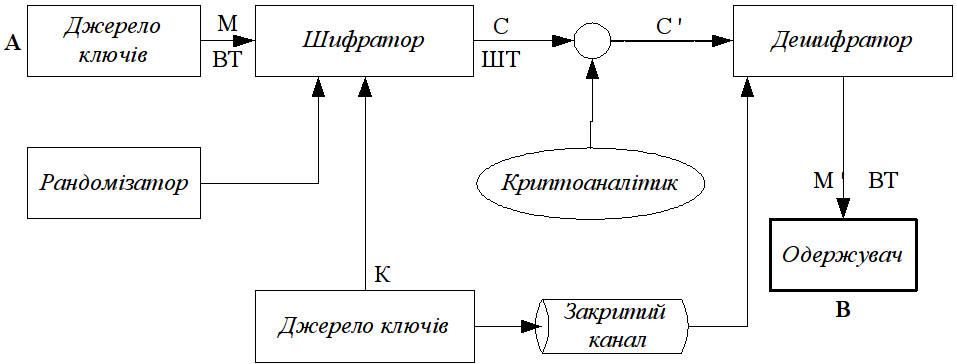
\includegraphics[width=5.0in]{crypt-img/crypt-img4.png}
    \caption{Загальна схема секретного зв'язку}\label{img:secretConnection}
\end{figure}

\input{lecture04.tex}
\input{lecture05.tex}
\input{lecture06.tex}
\input{lecture07.tex}
\input{lecture08.tex}
\input{lecture09.tex}
\input{lecture10.tex}
\input{lecture11.tex}
\input{lecture12.tex}
\input{lecture13.tex}
\input{lecture14.tex}
\input{lecture15.tex}
\input{lecture16.tex}
\input{lecture17.tex}
\input{lecture18.tex}

\bibliographystyle{../utf8gost705u}
\bibliography{bibliography}
\printindex
\tableofcontents
\end{document}
